% ============================================================
% 32-bezier-symbolic-explained.tex
% Compile with:  pdflatex -shell-escape 32-bezier-symbolic-explained.tex
% Both PNGs must be in the same folder. Run twice for TOC.
% ============================================================

\documentclass[12pt, a4paper]{article}

\usepackage[T1]{fontenc}
\usepackage[utf8]{inputenc}
\usepackage{lmodern}
\usepackage[top=2.5cm, bottom=2.5cm, left=2.8cm, right=2.8cm]{geometry}
\usepackage{graphicx}
\usepackage{float}
\usepackage[dvipsnames]{xcolor}

\definecolor{codebg}{RGB}{248,248,248}
\definecolor{rulecolor}{RGB}{180,180,180}
\definecolor{examplebg}{RGB}{240,248,255}
\definecolor{examplerule}{RGB}{100,149,237}
\definecolor{notebg}{RGB}{255,250,230}
\definecolor{noterule}{RGB}{210,180,50}
\definecolor{samebg}{RGB}{245,245,245}
\definecolor{samerule}{RGB}{160,160,160}

\usepackage{minted}
\setminted[julia]{
  bgcolor=codebg, frame=leftline, framerule=1.5pt,
  rulecolor=rulecolor, linenos=false, fontsize=\small,
  breaklines=true, tabsize=4, style=friendly,
}

\usepackage{amsmath}
\usepackage{amssymb}
\usepackage{mdframed}

\newmdenv[backgroundcolor=examplebg, linecolor=examplerule,
  linewidth=1.5pt, leftline=true, rightline=false,
  topline=false, bottomline=false,
  innerleftmargin=10pt, innerrightmargin=8pt,
  innertopmargin=6pt, innerbottommargin=6pt,
  skipabove=6pt, skipbelow=4pt]{examplebox}

\newmdenv[backgroundcolor=notebg, linecolor=noterule,
  linewidth=1.5pt, leftline=true, rightline=false,
  topline=false, bottomline=false,
  innerleftmargin=10pt, innerrightmargin=8pt,
  innertopmargin=6pt, innerbottommargin=6pt,
  skipabove=6pt, skipbelow=4pt]{notebox}

\newmdenv[backgroundcolor=samebg, linecolor=samerule,
  linewidth=1.5pt, leftline=true, rightline=false,
  topline=false, bottomline=false,
  innerleftmargin=10pt, innerrightmargin=8pt,
  innertopmargin=6pt, innerbottommargin=6pt,
  skipabove=6pt, skipbelow=4pt]{samebox}

\usepackage[colorlinks=true, linkcolor=black, urlcolor=MidnightBlue]{hyperref}
\usepackage{booktabs}
\usepackage{needspace}
\usepackage{parskip}
\usepackage{titlesec}
\usepackage{fancyhdr}
\usepackage{datetime2}

\titleformat{\section}
  {\large\bfseries\color{MidnightBlue}}{\thesection.}{0.6em}{}
  [\vspace{-4pt}\rule{\linewidth}{0.4pt}]
\titleformat{\subsection}
  {\normalsize\bfseries\color{BrickRed}}{\thesubsection.}{0.5em}{}
\titleformat{\subsubsection}
  {\normalsize\bfseries}{\thesubsubsection.}{0.5em}{}

\pagestyle{fancy}
\fancyhf{}
\rhead{\textcolor{gray}{\small 32-bezier-symbolic-explained}}
\lhead{\textcolor{gray}{\small B\'ezier Symbolic --- GLMakie}}
\cfoot{\thepage}
\renewcommand{\headrulewidth}{0.3pt}

\newcommand{\cd}[1]{\texttt{#1}}

\title{%
  \vspace{1cm}
  {\LARGE\bfseries B\'ezier Curve: Generic + Symbolic}\\[0.4em]
  {\large GLMakie + Symbolics.jl}\\[0.4em]
  {\large Code and Plot Explanation for Julia Beginners}\\[0.4em]
  {\normalsize\texttt{32-bezier-symbolic.jl}}
}
\author{E.R.\ Nurwijayadi}
\date{\DTMtoday}

\begin{document}

\maketitle
\thispagestyle{empty}

\begin{center}
\textit{Directed and curated by E.R.\ Nurwijayadi.
Code and explanations AI-generated.}
\end{center}

\begin{center}
\begin{minipage}{0.85\textwidth}
\small
This document explains \cd{32-bezier-symbolic.jl}.
It is the symbolic counterpart to \cd{31-bezier-generic.jl}:
the same generic curve and drawing code, with one difference ---
curve points are computed via \textbf{Symbolics.jl} instead
of direct Bernstein evaluation.
The polynomial is built once as a symbolic expression,
then evaluated by substitution.
This document focuses entirely on what changed.
Everything else is documented in \cd{31-bezier-generic-explained}.
\end{minipage}
\end{center}

\vspace{1em}\hrule\vspace{1.5em}
\tableofcontents
\newpage


% =============================================================
\needspace{8\baselineskip}
\section{The Two Plots}
% =============================================================

\needspace{5\baselineskip}
\subsection{Case 1 --- Quadratic 2-D}

\begin{figure}[H]
  \centering
  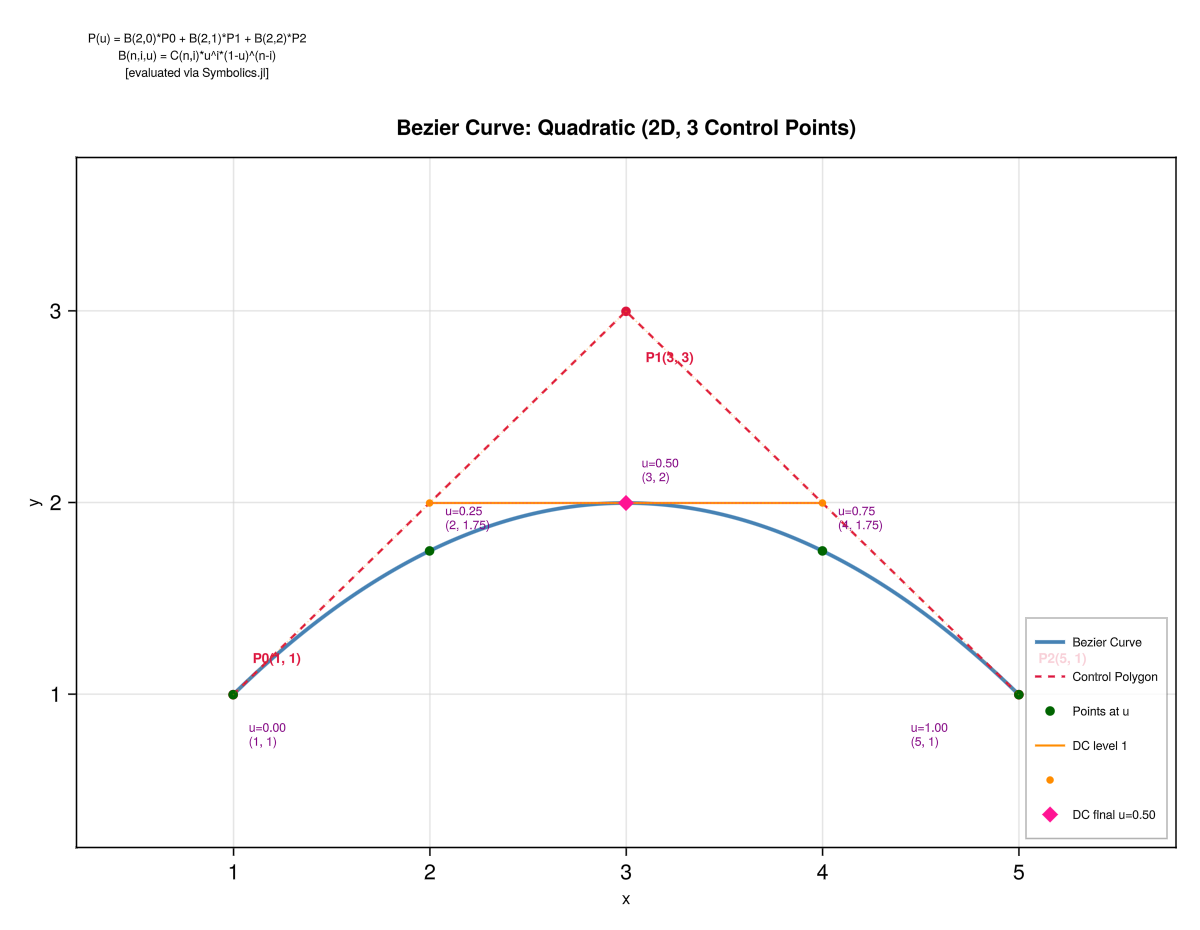
\includegraphics[width=0.92\linewidth]{32-bezier-quadratic-2d.png}
  \caption{Case~1: quadratic B\'ezier in 2-D.
           Note the equation label now includes
           \cd{[evaluated via Symbolics.jl]}.}
\end{figure}

\needspace{5\baselineskip}
\subsection{Case 2 --- Quartic 3-D}

\begin{figure}[H]
  \centering
  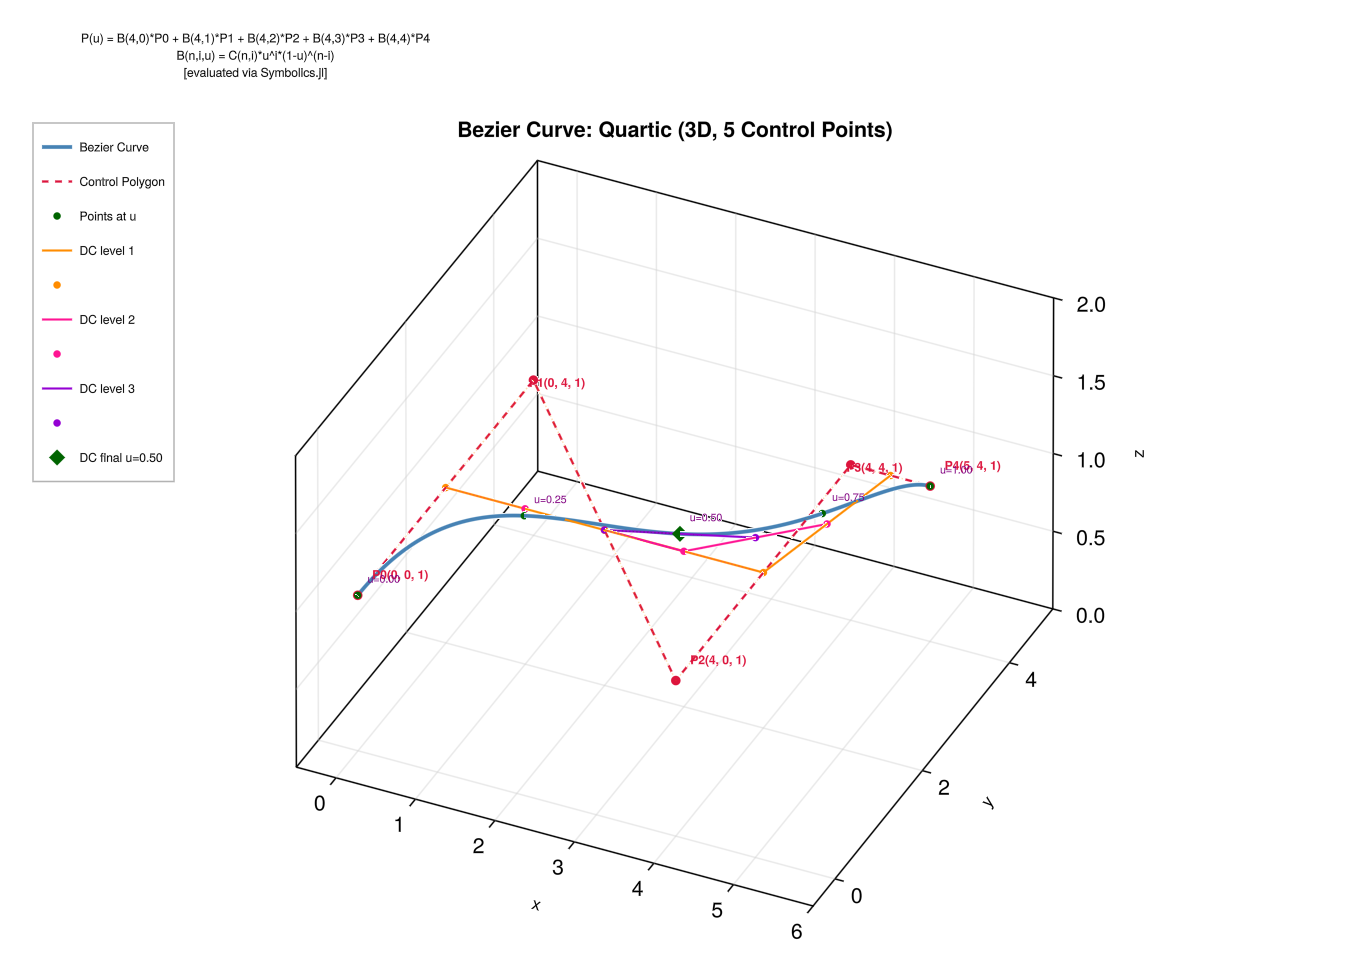
\includegraphics[width=0.92\linewidth]{32-bezier-quartic-3d.png}
  \caption{Case~2: quartic B\'ezier in 3-D.
           Visually identical to script~31.}
\end{figure}

The plots are visually identical to script~31.
The only visible difference is the third line in the
equation label: \cd{[evaluated via Symbolics.jl]}.


% =============================================================
\needspace{8\baselineskip}
\section{What Is Identical to Script 31}
% =============================================================

\begin{samebox}
\begin{tabular}{lp{9.5cm}}
\toprule
Component & Note \\
\midrule
\cd{CASE\_DATA} & Identical --- same points, $u$ values, filenames. \\
\cd{BezierCurve} struct \& constructor & Identical. \\
\cd{degree\_name}, \cd{dim\_name} & Identical. \\
\cd{de\_casteljau} & Identical --- generic \cd{while} loop. \\
All colour constants & Identical. \\
\cd{draw\_and\_save} body & Identical --- same \cd{is\_3d} branching,
  same drawing layers, same De Casteljau loop,
  same auto-limits, same legend. \\
\cd{Label} equation box & Nearly identical: one added line
  \cd{[evaluated via Symbolics.jl]}. \\
\bottomrule
\end{tabular}
\end{samebox}


% =============================================================
\needspace{8\baselineskip}
\section{What Changed: The Symbolic Engine}
% =============================================================

\textit{Script~31 used a simple numeric Bernstein formula.
Script~32 replaces that with a two-step approach:
build the polynomial symbolically once, then evaluate
by substituting $u$ values.}

\begin{center}
\begin{tabular}{lll}
\toprule
Component & Script 31 & Script 32 \\
\midrule
Symbolic variable & none & \cd{@variables u\_sym} \\
Polynomial construction & none & \cd{build\_symbolic\_poly(bz)} \\
\cd{bz\_point} signature &
  \cd{(bz, u)} &
  \cd{(bz, polys, u)} \\
Evaluation method &
  Direct Bernstein formula &
  \cd{substitute(p, Dict(u\_sym => u))} \\
\cd{bz\_curve} / \cd{bz\_highlight} &
  \cd{(bz, n\_pts)} &
  \cd{(bz, polys, n\_pts)} \\
\cd{draw\_and\_save} signature &
  \cd{(bz, u\_highlight, u\_dc, filename)} &
  \cd{(bz, polys, u\_highlight, u\_dc, filename)} \\
\cd{main()} &
  Direct call &
  Builds \cd{polys}, prints them, then calls \cd{draw\_and\_save} \\
\bottomrule
\end{tabular}
\end{center}


% =============================================================
\needspace{8\baselineskip}
\section{The Symbolic Variable}
% =============================================================

\begin{minted}{julia}
@variables u_sym
\end{minted}

Creates a symbolic variable named \cd{u\_sym} using
Symbolics.jl.
It is named \cd{u\_sym} rather than \cd{u} to avoid
any possible collision with local numeric variable names
inside loops.
This symbolic variable is declared at module level ---
outside all functions --- so every function in the
script can use it.

\begin{notebox}
\textbf{Why \cd{u\_sym} and not \cd{u}?}
In scripts~12 and~22, \cd{@variables u} declared a
symbolic \cd{u}, which caused loop variables in
comprehensions to be renamed to \cd{u\_val} to avoid
shadowing.
Using \cd{u\_sym} from the start sidesteps this naming
conflict cleanly --- numeric loop variables can freely
use \cd{u} without any risk of confusion.
\end{notebox}


% =============================================================
\needspace{8\baselineskip}
\section{\texttt{build\_symbolic\_poly} --- One Polynomial per Dimension}
% =============================================================

\begin{minted}{julia}
function build_symbolic_poly(bz::BezierCurve)
    n = bz.degree
    [
        sum(
            binomial(n, i-1) * u_sym^(i-1) * (1 - u_sym)^(n-(i-1))
              * bz.points[i, d]
            for i in 1:bz.n
        )
        for d in 1:bz.dim
    ]
end
\end{minted}

This function builds the B\'ezier polynomial as a
symbolic expression for each spatial dimension.

\textbf{Structure:} a nested list comprehension.
The outer loop \cd{for d in 1:bz.dim} iterates over
dimensions ($x$, $y$, and optionally $z$).
The inner \cd{sum(...for i...)} accumulates the weighted
Bernstein terms for that dimension.

\textbf{Each term:}
\cd{binomial(n, i-1)} is the binomial coefficient ---
an exact integer from Julia's built-in function.
\cd{u\_sym\^{}(i-1)} is a symbolic power of \cd{u\_sym}.
\cd{(1 - u\_sym)\^{}(n-(i-1))} is another symbolic power.
\cd{bz.points[i, d]} is the scalar coordinate --- a
\cd{Float64} that gets multiplied into the symbolic expression.

The result is a \cd{Vector} of symbolic expressions,
one per dimension.
This vector is computed \emph{once} and passed to all
evaluation functions.

\begin{examplebox}
\textbf{For Case~1 (quadratic 2-D), \cd{build\_symbolic\_poly} returns:}

\medskip
\cd{polys[1]} (the $x$ polynomial, before expansion):

$\binom{2}{0}(1{-}u_\text{sym})^2 \cdot 1
 + \binom{2}{1}\,u_\text{sym}(1{-}u_\text{sym}) \cdot 3
 + \binom{2}{2}\,u_\text{sym}^2 \cdot 5$

After simplification by Symbolics.jl:
$x(u) = 1 + 4u$

\medskip
\cd{polys[2]} (the $y$ polynomial, before expansion):

$\binom{2}{0}(1{-}u_\text{sym})^2 \cdot 1
 + \binom{2}{1}\,u_\text{sym}(1{-}u_\text{sym}) \cdot 3
 + \binom{2}{2}\,u_\text{sym}^2 \cdot 1$

After simplification: $y(u) = -4u^2 + 4u + 1$

\medskip
Both are stored as \emph{unevaluated} Symbolics.jl
expressions --- no numeric $u$ has been substituted yet.
\end{examplebox}

\begin{notebox}
\textbf{Why build the polynomial once and reuse it?}

In script~31, every call to \cd{bz\_point(bz, u)} computed
$\sum B(n,i,u) \cdot P_i$ from scratch --- all the
powers, binomials, and multiplications, for every single $u$.

In script~32, \cd{build\_symbolic\_poly} constructs the
polynomial expression once.
Evaluating at 300 $u$ values for the curve then requires
300 substitution calls on the pre-built expression,
rather than 300 fresh Bernstein computations.
The symbolic representation encodes the full polynomial
structure, and substitution is a simple variable replacement.

For a quartic 3-D curve with 5 control points and
300 sample points, this means building 3 symbolic
expressions once, then doing 900 substitutions,
rather than $300 \times 5 \times 3 = 4500$ full
Bernstein computations.
\end{notebox}


% =============================================================
\needspace{8\baselineskip}
\section{\texttt{bz\_point} --- Evaluation by Substitution}
% =============================================================

\begin{minted}{julia}
function bz_point(bz::BezierCurve, polys::Vector, u::Float64)
    [Float64(Symbolics.value(substitute(p, Dict(u_sym => u))))
     for p in polys]
end
\end{minted}

For each symbolic polynomial \cd{p} in \cd{polys},
this substitutes the numeric value \cd{u} for the
symbolic variable \cd{u\_sym} and extracts a
\cd{Float64} result.

\textbf{\cd{substitute(p, Dict(u\_sym => u))}:}
Replaces every occurrence of \cd{u\_sym} in the
expression \cd{p} with the numeric value \cd{u}.
Returns a Symbolics.jl expression that simplifies to
a number (but is still wrapped in the Symbolics type).

\textbf{\cd{Symbolics.value(...)}}:
Unwraps the Symbolics wrapper and returns the underlying
numeric value (a \cd{SymbolicUtils} numeric type).

\textbf{\cd{Float64(...)}:}
Converts the result to a plain Julia \cd{Float64}.

\begin{examplebox}
\textbf{Evaluating $x(0.5)$ for Case~1:}

\cd{p = polys[1]} represents $1 + 4u_\text{sym}$.

\cd{substitute(p, Dict(u\_sym => 0.5))}
$\to$ Symbolics expression for $1 + 4 \times 0.5 = 3$

\cd{Symbolics.value(...)} $\to$ \cd{3} (numeric)

\cd{Float64(3)} $\to$ \cd{3.0}

The full \cd{bz\_point} call for $u=0.5$ returns
\cd{[3.0, 2.0]} --- same as script~31. \checkmark
\end{examplebox}

\begin{notebox}
\textbf{Compared to script~31's \cd{bz\_point}:}

Script~31:
\begin{minted}{julia}
function bz_point(bz::BezierCurve, u::Float64)
    sum(bernstein(bz.degree, i-1, u) .* bz.points[i,:]
        for i in 1:bz.n)
end
\end{minted}

Script~32:
\begin{minted}{julia}
function bz_point(bz::BezierCurve, polys::Vector, u::Float64)
    [Float64(Symbolics.value(substitute(p, Dict(u_sym => u))))
     for p in polys]
end
\end{minted}

Script~31 takes two arguments (\cd{bz} and \cd{u}) and
computes the Bernstein formula directly.
Script~32 takes three arguments (\cd{bz}, \cd{polys},
and \cd{u}) and evaluates pre-built symbolic expressions.
Both return a length-\cd{dim} vector of coordinates.
The \cd{polys} argument propagates through
\cd{bz\_curve} and \cd{bz\_highlight} in the same way.
\end{notebox}


% =============================================================
\needspace{8\baselineskip}
\section{\texttt{main()} --- Printing the Polynomials}
% =============================================================

\begin{minted}{julia}
function main()
    data  = CASE_DATA[CASE]
    bz    = BezierCurve(data.points)
    println("Building symbolic polynomials...")
    polys = build_symbolic_poly(bz)
    println("Polynomials:")
    for (d, axis) in enumerate(bz.dim == 3 ? ["x","y","z"] : ["x","y"])
        println("  $(axis)(u) = $(expand(polys[d]))")
    end
    draw_and_save(bz, polys, data.u_highlight, data.u_dc, data.output)
end
\end{minted}

Script~32's \cd{main} does something script~31 did not:
it prints the symbolic polynomials to the terminal
before drawing the plot.

\textbf{\cd{expand(polys[d])}:}
Calls Symbolics.jl's \cd{expand()} on the symbolic
expression to fully distribute and collect terms.
This produces the clean monomial form for display ---
the same polynomials computed algebraically in scripts~01--05.

\textbf{The axis name list:}
\cd{bz.dim == 3 ? ["x","y","z"] : ["x","y"]} is a ternary
expression returning the appropriate axis name list for
2-D or 3-D.

\begin{examplebox}
\textbf{Terminal output for Case~1 (\cd{CASE=1}):}
\begin{minted}{text}
Building symbolic polynomials...
Polynomials:
  x(u) = 1 + 4u_sym
  y(u) = 1 + 4u_sym - 4(u_sym^2)
\end{minted}

\textbf{Terminal output for Case~2 (\cd{CASE=2}):}
\begin{minted}{text}
Building symbolic polynomials...
Polynomials:
  x(u) = (24//1)*(u_sym^2) - (32//1)*(u_sym^3) + (13//1)*(u_sym^4)
  y(u) = (16//1)*u_sym - (48//1)*(u_sym^2) + ...
  z(u) = 1
\end{minted}

These are the exact same polynomials from scripts~01--05,
now derived symbolically from the control points.
The \cd{u\_sym} in the output is the name of the
symbolic variable as declared.
\end{examplebox}


% =============================================================
\needspace{8\baselineskip}
\section{The Equation Label}
% =============================================================

\begin{minted}{julia}
eq = "P(u) = $terms\nB(n,i,u) = C(n,i)*u^i*(1-u)^(n-i)\n[evaluated via Symbolics.jl]"
\end{minted}

The only visible difference in the plots is this third
line in the equation label: \cd{[evaluated via Symbolics.jl]}.
It signals to the reader that the curve was not computed
by direct Bernstein arithmetic but through symbolic
polynomial evaluation.
The label is otherwise identical to script~31.


% =============================================================
\needspace{8\baselineskip}
\section{Summary: Script 31 vs Script 32}
% =============================================================

\begin{center}
\begin{tabular}{lp{5cm}p{5cm}}
\toprule
Aspect & Script 31 & Script 32 \\
\midrule
Evaluation engine &
  Direct Bernstein formula per point &
  Symbolic polynomial built once, then substituted \\[4pt]
Symbolic variable &
  None &
  \cd{@variables u\_sym} \\[4pt]
Key new function &
  \cd{bernstein(n,i,u)} &
  \cd{build\_symbolic\_poly(bz)} \\[4pt]
\cd{bz\_point} method &
  \cd{(bz, u)} &
  \cd{(bz, polys, u)} \\[4pt]
Terminal output &
  None beyond progress messages &
  Prints the expanded polynomial per axis \\[4pt]
Equation label &
  Two lines &
  Three lines: adds \cd{[evaluated via Symbolics.jl]} \\[4pt]
Plot appearance &
  Identical to script~32 &
  Identical to script~31 \\
\bottomrule
\end{tabular}
\end{center}

\begin{notebox}
\textbf{Which should you use?}

Script~31 is simpler and faster to understand ---
the evaluation is explicit arithmetic you can trace
by hand.

Script~32 is more powerful for exploration ---
\cd{build\_symbolic\_poly} gives you the full polynomial
expression that you can inspect, differentiate, or
manipulate before evaluating.
The terminal printout of the polynomials is itself
useful: it confirms that the control points produce
the expected algebraic form.

\textit{Script~31 computes the curve.
Script~32 also \emph{understands} it.}
\end{notebox}

\vspace{2em}\hrule\vspace{0.5em}
{\small\textcolor{gray}{%
Explanation for \texttt{32-bezier-symbolic.jl}
\textbar{} Directed and curated by E.R.\ Nurwijayadi
\textbar{} Code and explanations AI-generated}}

\end{document}
